\begin{commands}[]{}
\bgroup
\makeatletter
\fboxrule0px
\fboxsep-0px
\parindent0pt
\sffamily
\mbox{}%
\centerline{\huge\bfseries \mainhead@cx}%
\vskip2\baselineskip
\makedoublehead%
\hfill\hfill\fbox{\begin{minipage}[t]{0.55\textwidth}%
\null%
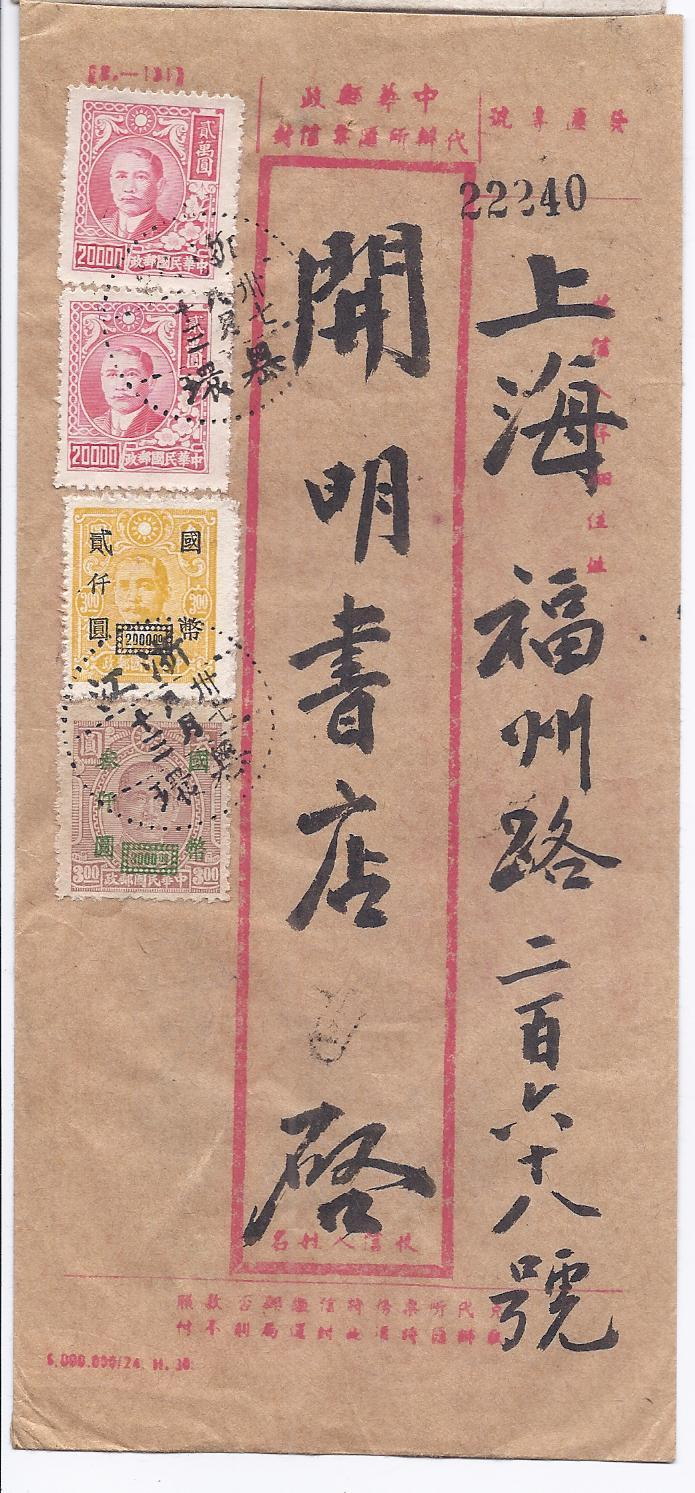
\includegraphics[width=1.01\linewidth]{./images/1948-02.jpg}%
\vspace*{20pt}
\end{minipage}}\hfil%
\fbox{\begin{minipage}[t]{.4\linewidth}%
\fbox{\begin{minipage}[t]{\textwidth}%
\null
\lipsum[1]
\end{minipage}}%
\par
\leavevmode\vskip0pt\rule{1px}{30px}\vskip0pt
\fbox{\begin{minipage}[t]{\textwidth}%
\null
\lipsum[1]
\end{minipage}}%
\end{minipage}}%\hfill
\par
\leavevmode
\bfseries The bottom part of the description, would normally go here. This is textbox3 and the text can just be entered by typing in the environment. Any language can be used and also footnote as for example\footnote{Footnote example.}.
\egroup
\end{commands}

\begin{commands}[]{}
\begin{verbatim}
\bgroup
\makeatletter
\fboxrule0px
\fboxsep0px
\parindent0pt
\sffamily
\mbox{}%
\centerline{\huge\bfseries \mainhead@cx}%
\vskip2\baselineskip
\makedoublehead
\centering
\hfill\hfill\fbox{\begin{minipage}[t]{0.55\textwidth}%
\null
\centering
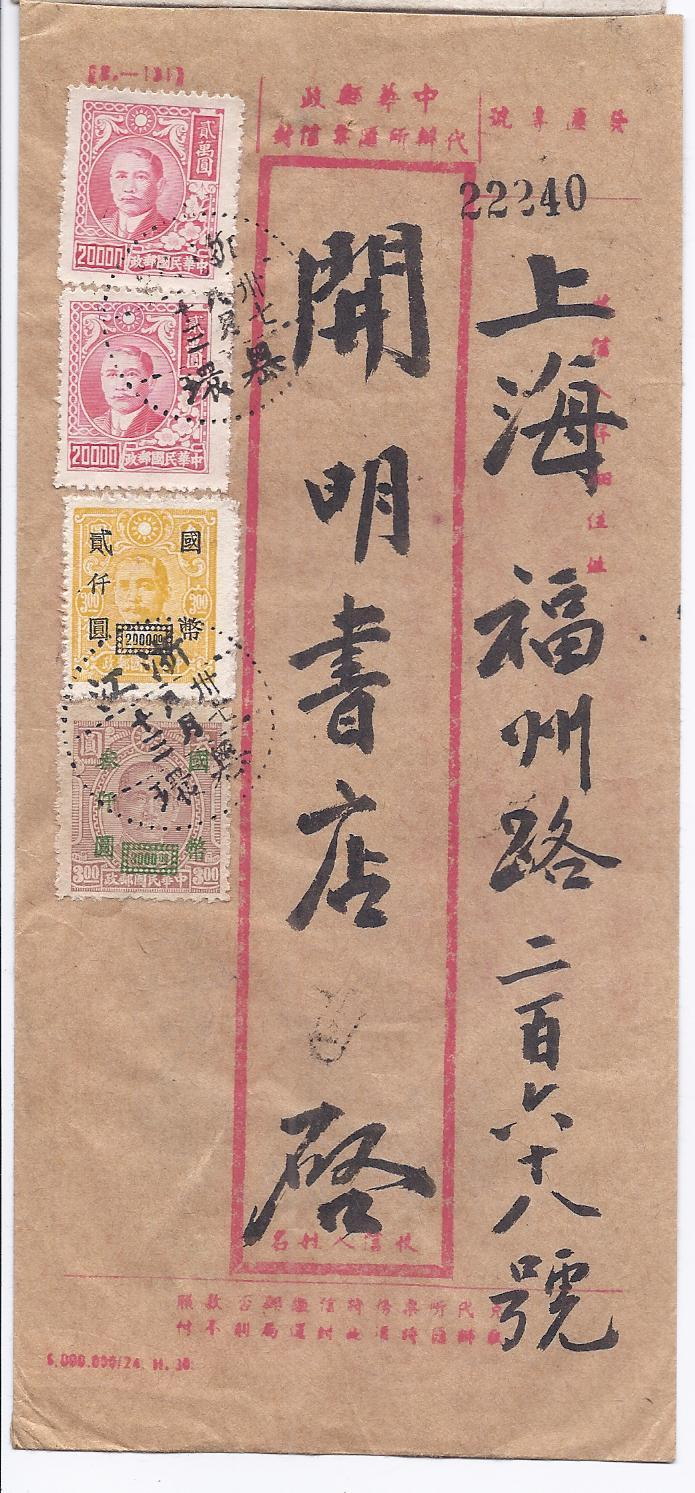
\includegraphics[width=1.03\linewidth]{./images/1948-02.jpg}%
\vspace*{20pt}
\end{minipage}}\hfil%
\fbox{\begin{minipage}[t]{.4\linewidth}%
\fbox{\begin{minipage}[t]{\textwidth}%
\null
\lipsum[1]
\end{minipage}}%
\par
\leavevmode\vskip0pt\rule{1px}{30px}\vskip0pt
\fbox{\begin{minipage}[t]{\textwidth}%
\null
\lipsum[1]
\end{minipage}}%
\end{minipage}}%\hfill
\par
\leavevmode
\bfseries The bottom part of the description, would normally go here... 
 example\footnote{Footnote example.}.
\egroup
\end{verbatim}
\end{commands}